\documentclass[aspectratio=169,12pt]{beamer}

% ---------------------------------------------------------------------------
% Mid-Semester Evaluation: Reliability-Weighted Ensembling for Cross-Domain
% LLM Session Recommendation
%
% 25 frames (including title).
%
% THIS VERSION: language simplified to plain English throughout.
% Nothing added, nothing removed -- same frames, same order, same meaning.
% Most frames got SHORTER, so there is more breathing room than before.
% ---------------------------------------------------------------------------

\usetheme{Boadilla}
\usecolortheme{dove}
\usefonttheme{professionalfonts}
\setbeamertemplate{navigation symbols}{}

\usepackage[T1]{fontenc}
\usepackage[utf8]{inputenc}
\usepackage{amsmath,amssymb}
\usepackage{array,booktabs,tabularx,multirow}
\usepackage{graphicx}
\usepackage{hyperref}
\usepackage{ragged2e}
\usepackage{xcolor}
\usepackage{tikz}
\usetikzlibrary{arrows.meta,calc,fit,positioning,shapes.geometric}

% Palette
\definecolor{DeepBlue}{HTML}{143D59}
\definecolor{Teal}{HTML}{087E8B}
\definecolor{Orange}{HTML}{F28F3B}
\definecolor{SoftBlue}{HTML}{EAF2F8}
\definecolor{SoftTeal}{HTML}{E8F6F3}
\definecolor{SoftOrange}{HTML}{FFF3E8}
\definecolor{Ink}{HTML}{263238}
\definecolor{Muted}{HTML}{607D8B}
\definecolor{LightGray}{HTML}{D9E2E8}

\setbeamercolor{structure}{fg=DeepBlue}
\setbeamercolor{normal text}{fg=Ink,bg=white}
\setbeamercolor{frametitle}{fg=DeepBlue,bg=SoftBlue}
\setbeamercolor{title}{fg=DeepBlue}
\setbeamercolor{subtitle}{fg=Muted}
\setbeamercolor{block title}{fg=white,bg=DeepBlue}
\setbeamercolor{block body}{fg=Ink,bg=SoftBlue}
\setbeamercolor{block title alerted}{fg=white,bg=Orange}
\setbeamercolor{block body alerted}{fg=Ink,bg=SoftOrange}
\setbeamercolor{block title example}{fg=white,bg=Teal}
\setbeamercolor{block body example}{fg=Ink,bg=SoftTeal}
\setbeamerfont{frametitle}{series=\bfseries,size=\Large}
\setbeamerfont{title}{series=\bfseries,size=\Huge}
\setbeamerfont{subtitle}{size=\large}

\setbeamertemplate{footline}{%
  \leavevmode%
  \hbox{%
    \begin{beamercolorbox}[wd=.82\paperwidth,ht=2.6ex,dp=1.1ex,leftskip=1em]{author in head/foot}%
      \usebeamerfont{author in head/foot}\insertshorttitle
    \end{beamercolorbox}%
    \begin{beamercolorbox}[wd=.18\paperwidth,ht=2.6ex,dp=1.1ex,center]{date in head/foot}%
      \usebeamerfont{date in head/foot}\insertframenumber/\inserttotalframenumber
    \end{beamercolorbox}}%
}

\newcommand{\source}[1]{\vspace{0.35em}\par{\tiny\color{Muted}\textit{#1}}}
\newcommand{\key}[1]{\textcolor{Teal}{\textbf{#1}}}
\newcommand{\warn}[1]{\textcolor{Orange}{\textbf{#1}}}
\newcommand{\code}[1]{\texttt{\footnotesize #1}}

\title[RWRA for Cross-Domain LLM SR]{Reliability-Weighted Ensembling for\\Cross-Domain LLM Session Recommendation}
\subtitle{Research Progress Presentation}
\author{Swaral Gaur}
\institute{Computer Science Engineering / Dr. B. R. Ambedkar National Institute of Technology Jalandhar}
\date{\today}

\begin{document}

% ============================================================ Frame 1
\begin{frame}[plain]
\centering
\vspace{0.5cm}
{\color{DeepBlue}\bfseries\LARGE
Reliability-Weighted Ensembling for\par}
{\color{DeepBlue}\bfseries\LARGE
Cross-Domain LLM Session Recommendation\par}
\vspace{0.4cm}
{\color{Muted}\large Research Progress Presentation\par}
\vfill
{\normalsize Presented by\par}
\vspace{0.1cm}
{\large\bfseries Swaral Gaur\par}
{\normalsize Computer Science Engineering\par}
\vspace{0.4cm}
{\normalsize Under the supervision of\par}
\vspace{0.1cm}
{\large\bfseries Mrs. Naina Yadav\par}
{\normalsize Department of Computer Science and Engineering\par}
\vspace{0.4cm}
{\normalsize Dr. B. R. Ambedkar National Institute of Technology Jalandhar\par}
\vspace{0.15cm}
{\normalsize \today\par}
\end{frame}

% ============================================================ Frame 2
\begin{frame}{Presentation roadmap}
\begin{enumerate}
  \item The problem: why AI recommenders are not yet reliable.
  \item What other researchers have already done.
  \item The gap I am filling.
  \item My approach, and the full pipeline.
  \item The method: agreement-based and history-based weighting.
  \item How I will test it.
  \item Where I stand today.
  \item Conclusion and next steps.
\end{enumerate}
\end{frame}

% ============================================================ Frame 3
\begin{frame}{Problem statement I -- the core problem}
\begin{alertblock}{Central problem}
Ask an AI recommender the same question in different words, and it gives a
\emph{different answer} -- same user, same options, same model. Only the
wording changed.
\end{alertblock}

\vspace{0.6em}
\begin{itemize}
  \item AI recommenders like PO4ISR report good accuracy. But nobody checks
        whether that accuracy survives a different wording, a different
        kind of data, or a smaller model.
  \item One accuracy number cannot tell you whether the system is
        \emph{trustworthy}, or whether you just got \emph{lucky with the
        wording you happened to choose}.
\end{itemize}
\end{frame}

% ============================================================ Frame 4
\begin{frame}{Problem statement II -- why it matters, and the question}
\begin{itemize}
  \item The two existing fixes need either a huge commercial AI (such as
        Gemini), or a \emph{second} system that you have to train yourself.
  \item Neither has been tried on a small AI running on an ordinary
        machine -- which is what most students and most companies actually
        have.
\end{itemize}

\vspace{0.8em}
\begin{block}{The question behind this work}
Can we make an AI recommender more reliable using only that one small AI --
no huge model, no second trained system -- and does the fix still work when
we move to a different kind of data?
\end{block}
\end{frame}

% ============================================================ Frame 5
\begin{frame}{Background: how recommendation works, and what breaks}
\begin{columns}[T]
\column{0.48\linewidth}
\begin{block}{Session-based recommendation}
\begin{itemize}
  \item Guess what a user will pick next, using only what they did in this
        one visit.
  \item Older systems (GRU4Rec, SASRec, BERT4Rec) turn each item into a
        list of numbers.
  \item AI language models instead \emph{read} the item names and reason
        about them in plain words.
\end{itemize}
\end{block}

\column{0.48\linewidth}
\begin{alertblock}{What changes with an AI model}
\begin{itemize}
  \item The answer now depends on \emph{how you ask}, not only on the data
        you give it.
  \item With a long history, the AI can lose track of what matters. This is
        called \emph{semantic drift}.
  \item Item names containing numbers (``Xbox 360'') can be mistaken for
        rank numbers when reading the answer.
\end{itemize}
\end{alertblock}
\end{columns}

\vspace{0.6em}
\centering
\Large\textcolor{DeepBlue}{Reliability is something you measure and build -- not something you assume.}
\end{frame}

% ============================================================ Frame 6
\begin{frame}{Literature review I -- reproducibility and semantic drift}
\begin{block}{Tiwari, Rekha \& Mundotiya (2026) -- arXiv:2605.18780}
\emph{A Reproducibility Analysis of PO4ISR: Diagnosing and Mitigating
Semantic Drift in LLM-Based Session Recommendation}
\end{block}

\begin{columns}[T]
\column{0.48\linewidth}
\textbf{What they found}
\begin{itemize}
  \item Re-ran PO4ISR (Sun et al., 2024) on movies, games and bundles.
  \item The output is unstable, and a prompt tuned on one kind of data
        fails on another.
\end{itemize}

\column{0.48\linewidth}
\textbf{Their fix -- PO4ISR++}
\begin{itemize}
  \item Make the AI output position numbers, which removes the
        number-confusion problem.
  \item Combine prompts from different data types, using
        \textbf{Gemini-2.0} to do the combining.
  \item Big gains: up to 54\% (games) and 96\% (bundles).
\end{itemize}
\end{columns}

\vspace{0.5em}
\begin{alertblock}{Why this matters for my work}
Their fix needs a huge commercial AI to do the combining. They never test
it on a small model you could run yourself.
\end{alertblock}
\source{Tiwari, Rekha, and Mundotiya, arXiv:2605.18780v1, 2026.}
\end{frame}

% ============================================================ Frame 7
\begin{frame}{Literature review II -- Llama4Rec: how it works}
\begin{block}{Luo et al.\ (2026) -- IEEE JSTSP, Vol.\ 20, No.\ 1}
\emph{Integrating Large Language Models Into Recommendation via Mutual
Augmentation and Adaptive Aggregation (Llama4Rec)}
\end{block}

\vspace{0.6em}
\begin{itemize}
  \item They re-train LLaMA-2 (7B/13B) on \textbf{16 datacenter GPUs}.
  \item They mix the AI's score with the score from a \textbf{second system
        they train separately}.
  \item How much of each? It depends on how much data that user has:
        $\ell_u = \log(N(u){+}1)$, where $N(u)$ counts the user's past
        actions. Little data $\Rightarrow$ trust the AI more. Lots of data
        $\Rightarrow$ trust the older system more.
\end{itemize}
\end{frame}

% ============================================================ Frame 8
\begin{frame}{Literature review II -- Llama4Rec: results and limits}
\begin{block}{What they report}
Their method beats the best older systems by about 14\% on two
recommendation tasks and 3\% on a third, across MovieLens-100K,
MovieLens-1M and BookCrossing.
\end{block}

\vspace{0.5em}
\begin{alertblock}{Why this matters for my work}
Their mixing weight only looks at \emph{how much data a user has}. It never
checks whether the AI's own answers agree with each other. And it needs a
second system that must be trained and maintained. The authors themselves
call training at this scale \emph{``impractical''} for large or
resource-limited use.
\end{alertblock}
\source{Luo, Yao, He, Shao, Xu, Huang, Zhou, Zhang, Xiao, Hou, Zhan, and Song, IEEE JSTSP, 2026.}
\end{frame}

% ============================================================ Frame 9
\begin{frame}{Literature review III -- self-consistency and the gap}
\begin{columns}[T]
\column{0.46\linewidth}
\textbf{Wider background}
\begin{itemize}
  \item Self-consistency: ask the AI several times and take the majority
        answer. Well known for reasoning tasks, never tried on this drift
        problem.
  \item PREFER: combines several prompts by letting the AI review and
        improve them.
  \item Weighted combining exists in recommenders, but never based on
        whether the answers agree for that one user.
\end{itemize}

\column{0.46\linewidth}
\small
\begin{tabularx}{\linewidth}{@{}p{0.30\linewidth}X@{}}
\toprule
\textbf{Work} & \textbf{What it leaves open}\\
\midrule
PO4ISR++ & Needs a huge model to combine prompts\\
Llama4Rec & Needs a 2nd trained system; fixed weight\\
Self-consistency & Never tried on this problem\\
\bottomrule
\end{tabularx}
\end{columns}

\vspace{0.6em}
\begin{alertblock}{The gap I am filling}
Nobody has measured \emph{per-user} answer agreement, on a \emph{small
local} AI, with \emph{no second trained system}, across \emph{more than one
kind of data}.
\end{alertblock}
\end{frame}

% ============================================================ Frame 10
\begin{frame}{Research questions I}
\begin{block}{RQ1 -- How bad is the problem?}
If I change only the wording -- keeping the user, the options, the model
and the settings exactly the same -- how much does the answer change?
\end{block}

\vspace{0.8em}
\begin{block}{RQ2 -- Can I fix it?}
If I ask the \emph{same} small AI in four different ways and combine the
answers based on how much they agree, do I get the reliability the other
two papers needed a huge model or a second system for?
\end{block}
\end{frame}

% ============================================================ Frame 11
\begin{frame}{Research questions II}
\begin{block}{RQ3 -- Who benefits most?}
Does combining help most for users with very little history, which is what
Llama4Rec's logic would suggest?
\end{block}

\vspace{0.5em}
\begin{block}{RQ4 -- Does it travel?}
Does it work on both movies and video games, with no special tuning for
either?
\end{block}

\vspace{0.6em}
\begin{exampleblock}{My position in one sentence}
Paper one says \emph{use a bigger model}. Paper two says \emph{use a second
model}. I say: \emph{use more evidence from the same small model, weighted
by how much that evidence agrees with itself.}
\end{exampleblock}
\end{frame}

% ============================================================ Frame 12
\begin{frame}{My approach -- the full pipeline}
\centering
\resizebox{\linewidth}{!}{%
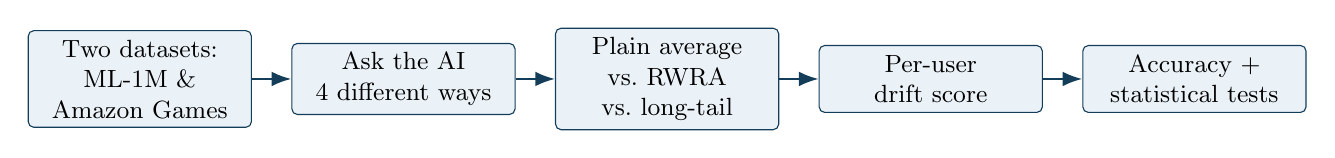
\begin{tikzpicture}[
  node distance=0.5cm,
  every node/.style={font=\small},
  stage/.style={draw=DeepBlue, rounded corners=2pt, fill=SoftBlue,
               minimum height=0.85cm, text width=2.6cm, align=center},
  arrow/.style={-{Latex[length=2.5mm]}, thick, DeepBlue}
]
\node[stage] (data) {Two datasets:\\ML-1M \& Amazon Games};
\node[stage, right=of data] (ens) {Ask the AI\\4 different ways};
\node[stage, right=of ens] (agg) {Plain average\\vs.\ RWRA\\vs.\ long-tail};
\node[stage, right=of agg] (drift) {Per-user\\drift score};
\node[stage, right=of drift] (eval) {Accuracy +\\statistical tests};
\draw[arrow] (data) -- (ens);
\draw[arrow] (ens) -- (agg);
\draw[arrow] (agg) -- (drift);
\draw[arrow] (drift) -- (eval);
\end{tikzpicture}}

\vspace{0.6em}
\begin{block}{The key design rule}
All four methods -- single prompt, plain average, Reliability-Weighted Rank
Aggregation (RWRA), and long-tail-weighted RWRA -- are tested on the
\emph{same} users and the \emph{same} options. Only the combining rule
changes.
\end{block}
\end{frame}

% ============================================================ Frame 13
\begin{frame}{Methodology -- the data and how I test}
\begin{table}
\centering
\small
\begin{tabular}{lrr}
\toprule
\textbf{Property} & \textbf{MovieLens-1M} & \textbf{Amazon Games}\\
\midrule
Users (one test each) & 6{,}040 & 94{,}762\\
Options per question & 20 & 20\\
Wrong options chosen by & popularity & popularity\\
Word used in the prompt & ``movie'' & ``game''\\
\bottomrule
\end{tabular}
\end{table}

\begin{itemize}
  \item For each user I hide their \emph{last} action and show the AI
        everything before it. The hidden one is the correct answer.
  \item The answer never appears in the history and is never labelled, so
        the AI cannot cheat.
  \item Amazon uses text IDs, so I convert them to numbers. The same code
        then handles both datasets.
  \item Testing all 94{,}762 Amazon users would take weeks, so I use a fair
        random sample -- the same size for both datasets.
\end{itemize}
\end{frame}

% ============================================================ Frame 14
\begin{frame}{Methodology -- how the AI must answer}
\begin{block}{The answer format}
The AI must fill in a fixed form: one score from 0 to 100 for each of the
20 options.
\vspace{0.3em}
\centerline{\code{\{"scores": [85, 42, 91, \ldots]\}}}
\end{block}

\vspace{0.5em}
\begin{itemize}
  \item \emph{My program} does the sorting, not the AI. Since the AI never
        writes item names, a product called ``Xbox 360'' can never be
        mistaken for rank number 360.
  \item If the AI breaks the format, I record it as a failed answer and
        keep the raw text. I never quietly fix it -- fixing it would hide
        the very problem I am measuring.
  \item Two different failures, counted separately: the answer was
        \emph{unreadable}, versus the answer was readable but \emph{wrong}.
\end{itemize}
\end{frame}

% ============================================================ Frame 15
\begin{frame}{Methodology -- RWRA Step 1: ask four times}
\begin{block}{The idea}
Instead of trusting one prompt, \emph{Reliability-Weighted Rank
Aggregation} (RWRA) asks the \emph{same} AI the same question in four
different wordings, then combines the answers.
\end{block}

\vspace{0.7em}
\begin{itemize}
  \item For each user, the AI scores the same 20 options four times, using
        four different wordings of the instruction.
  \item Everything else stays identical -- same user, same options, same
        model, same settings. Only the wording changes.
  \item This is one small model asked four times, not four different
        models. Nothing extra to train, nothing extra to maintain.
\end{itemize}
\end{frame}

% ============================================================ Frame 16
\begin{frame}{Methodology -- RWRA Step 2: decide who to trust}
\begin{block}{The rule}
Each answer's weight is how much it agrees with the other three, on
average. Kendall's $\tau$ is the standard way to measure that agreement.
\end{block}

\vspace{0.8em}
\[
w_i \;=\; \frac{\tau_i + 1}{\sum_j (\tau_j + 1)}, \qquad
\tau_i = \frac{1}{k-1}\sum_{j \neq i} \mathrm{KendallTau}(r_i, r_j)
\]

\vspace{0.8em}
\begin{itemize}
  \item Agreement runs from $-1$ (exactly opposite) to $+1$ (identical).
        Adding 1 keeps every weight at zero or above -- a negative weight
        would mean flipping an answer, which makes no sense.
  \item I never need to know the correct answer. The weights come only
        from comparing the four answers with each other.
\end{itemize}
\end{frame}

% ============================================================ Frame 17
\begin{frame}{Methodology -- RWRA: a worked example (correct answer = A)}
\small
\begin{table}
\centering
\begin{tabular}{clcr}
\toprule
\textbf{Answer} & \textbf{Scores (A, B, C, D)} & \textbf{Its ranking} & \textbf{Weight}\\
\midrule
1 & 55, 50, 45, 40 & A, B, C, D & 33.3\%\\
2 & 56, 51, 46, 41 & A, B, C, D & 33.3\%\\
3 & 54, 49, 44, 39 & A, B, C, D & 33.3\%\\
4 & 10, 20, 30, \textbf{100} & \textbf{D, C, B, A} & \textbf{0\%}\\
\bottomrule
\end{tabular}
\end{table}

\vspace{0.2em}
\begin{table}
\centering
\begin{tabular}{lccccl}
\toprule
& \textbf{A} & \textbf{B} & \textbf{C} & \textbf{D} & \textbf{Where A lands}\\
\midrule
Plain average & 43.75 & 42.50 & 41.25 & \textbf{55.00} & \warn{2nd}\\
RWRA & \textbf{55.00} & 50.00 & 45.00 & 40.00 & \key{1st}\\
\bottomrule
\end{tabular}
\end{table}

\vspace{0.3em}
\centering
\textcolor{Orange}{\textbf{A plain average picks the wrong item.}}\quad
\textcolor{Teal}{\textbf{Agreement-weighting picks the right one.}}
\end{frame}

% ============================================================ Frame 18
\begin{frame}{Methodology -- the drift score}
\begin{block}{What it is}
The same agreement check that sets the weights also gives a free
diagnostic: the average agreement across all four answers, for this one
user.
\end{block}

\vspace{0.7em}
\[
\text{drift}_s \;=\; \frac{2}{k(k-1)}\sum_{i<j} \mathrm{KendallTau}(r_i, r_j)
\]

\vspace{0.7em}
\begin{itemize}
  \item Close to $+1$: all four wordings agreed -- the AI was stable for
        this user.
  \item Low or negative: the four answers disagreed -- the AI was unstable
        here, so this recommendation deserves caution.
\end{itemize}

\vspace{0.4em}
\centering
\textcolor{DeepBlue}{One calculation, two uses: the weights \emph{and} the warning signal.}
\end{frame}

% ============================================================ Frame 19
\begin{frame}{Methodology -- long-tail weighting: the idea}
\begin{alertblock}{Borrowed from Llama4Rec}
Llama4Rec mixes an AI with a \emph{second system it trains}, and decides
the mix based on how little data the \emph{user} has.
\end{alertblock}

\vspace{0.8em}
\begin{block}{How I changed it}
I have only one AI, so I reuse the same idea differently. I mix the
\textbf{four-answer combination} with the \textbf{single original prompt},
and decide the mix based on how short \emph{this user's history} is -- not
on a second system's confidence.
\end{block}

\vspace{0.5em}
\centering
\textcolor{DeepBlue}{\emph{They mix two models, based on how much data a user has.}
$\;\longrightarrow\;$
\emph{I mix two ways of using one model, based on history length.}}
\end{frame}

% ============================================================ Frame 20
\begin{frame}{Methodology -- long-tail weighting: the formulas}
\[
\ell_s = \log(\text{history length}+1)
\]
\[
\beta_s = \max\!\left(\frac{\ell_{\max}-\ell_s}{\ell_{\max}-\ell_{\min}},\,\beta_2\right)\cdot\beta_1
\]
\[
\text{final score} \;=\; \beta_s \cdot \text{RWRA} \;+\; (1-\beta_s)\cdot \text{single prompt}
\]

\vspace{0.5em}
\begin{itemize}
  \item Short history $\Rightarrow$ bigger $\beta_s$ $\Rightarrow$ trust
        the four-answer combination more.
  \item Long history $\Rightarrow$ smaller $\beta_s$ $\Rightarrow$ one
        prompt is probably already good enough.
  \item $\ell_{\min}$ and $\ell_{\max}$ come from the whole dataset, so a
        user's weight never changes depending on which sample they land in.
\end{itemize}
\end{frame}

% ============================================================ Frame 21
\begin{frame}{How I will test it}
\begin{columns}[T]
\column{0.48\linewidth}
\textbf{Accuracy}
\begin{itemize}
  \item HR@1, HR@5, HR@10 -- was the correct item in the top 1, 5 or 10?
  \item NDCG@5, NDCG@10 -- same idea, but higher positions count more.
  \item The same code computes these for all four methods.
\end{itemize}

\textbf{Stability}
\begin{itemize}
  \item Average agreement between the four answers.
  \item How much their top-5 and top-10 lists overlap.
\end{itemize}

\column{0.48\linewidth}
\textbf{Is the difference real?}
\begin{itemize}
  \item Bootstrap test (2000 re-samples) -- checks whether a difference is
        real or just luck.
  \item Wilcoxon test -- a second, independent check.
  \item Only users where \emph{both} methods gave a usable answer are
        compared.
\end{itemize}

\textbf{Who benefits}
\begin{itemize}
  \item All four methods re-measured separately for short, medium and long
        histories. This answers RQ3 directly.
\end{itemize}
\end{columns}
\end{frame}

% ============================================================ Frame 22
\begin{frame}{Where I stand today}
\begin{block}{What is built}
\begin{itemize}
  \item The full system: data handling for both datasets, both combining
        methods, and the statistics code.
\end{itemize}
\end{block}

\vspace{0.4em}
\begin{alertblock}{What is \emph{not} done yet -- said plainly}
I have not yet run this at full scale with the real AI model. The only
real-model evidence so far is a tiny pilot (next slide). The full runs are
my immediate next step, once I have GPU access.
\end{alertblock}
\end{frame}

% ============================================================ Frame 23
\begin{frame}{Early pilot evidence -- not final results}
\begin{table}
\centering
\small
\begin{tabular}{lrrrrr}
\toprule
\textbf{Wording used} & \textbf{HR@1} & \textbf{HR@5} & \textbf{HR@10} & \textbf{NDCG@5} & \textbf{NDCG@10}\\
\midrule
baseline\_scores\_v1 & 0.20 & 0.20 & 0.40 & 0.200 & 0.263\\
wording\_direct\_v1 & 0.40 & 0.40 & 0.60 & 0.400 & 0.460\\
\bottomrule
\end{tabular}
\end{table}

\vspace{0.5em}
\begin{alertblock}{How to read this table}
Only \textbf{5 users} per row. I ran this just to check that the AI
produces readable output for each wording. It is far too small to prove
anything statistically. I show it only because it hints that the wording
problem is real: two wordings gave 0.20 and 0.40 on the same measure.
\end{alertblock}
\source{Qwen2.5-3B-Instruct via Ollama, temperature 0, top-p 1, fully repeatable settings.}
\end{frame}

% ============================================================ Frame 24
\begin{frame}{Conclusion I -- what this work contributes}
\begin{block}{What I am adding}
\begin{itemize}
  \item A way to make AI recommenders more reliable without a huge model
        and without a second trained system.
  \item A per-user number that shows instability directly, instead of
        guessing at it from an overall drop in accuracy.
  \item An extension borrowed openly from Llama4Rec, adapted to work with
        only one model.
  \item Testing on two very different datasets -- movies and games -- with
        no special tuning for either.
\end{itemize}
\end{block}
\end{frame}

% ============================================================ Frame 25
\begin{frame}{Conclusion II -- what comes next}
\begin{block}{My next steps}
\begin{enumerate}
  \item A small real test on both datasets.
  \item The full run on the sample, with proper statistics.
  \item Check whether users with short histories benefit most.
  \item Write everything up, including honest limitations.
\end{enumerate}
\end{block}

\vspace{1em}
\centering
\Large\textcolor{DeepBlue}{Same small model. More evidence, weighted by how much it agrees with itself.}
\end{frame}

% ============================================================ Frame 26
\begin{frame}{References}
\small
\begin{block}{[1] The paper that defines the problem}
A. Tiwari, K. N. L. Rekha, and R. K. Mundotiya, ``A Reproducibility
Analysis of PO4ISR: Diagnosing and Mitigating Semantic Drift in LLM-Based
Session Recommendation,'' \emph{arXiv preprint arXiv:2605.18780}, 2026.
\vspace{0.2em}
\par\textcolor{Muted}{\footnotesize \textbf{I use this for:} the semantic-drift
problem, and the fact that their fix depends on a frontier-scale model.}
\end{block}

\vspace{0.4em}
\begin{block}{[2] The paper I adapt my weighting idea from}
S. Luo, Y. Yao, B. He, W. Shao, J. Xu, Y. Huang, A. Zhou, X. Zhang,
Y. Xiao, H. Hou, M. Zhan, and L. Song, ``Integrating Large Language Models
Into Recommendation via Mutual Augmentation and Adaptive Aggregation,''
\emph{IEEE Journal of Selected Topics in Signal Processing}, vol. 20,
no. 1, pp. 77--89, Jan. 2026.
\vspace{0.2em}
\par\textcolor{Muted}{\footnotesize \textbf{I use this for:} the long-tail
weighting mechanism, which I adapt to a single-model setting.}
\end{block}

\vspace{0.3em}
{\footnotesize\textcolor{Muted}{Also named in this talk: Sun et al.\ (SIGIR 2024),
PO4ISR; Wang et al.\ (ICLR 2023), self-consistency; Hidasi et al.\ (ICLR 2016),
Kang \& McAuley (ICDM 2018), Sun et al.\ (CIKM 2019), classical session models.}}
\end{frame}

\end{document}
